\section{Overview}
\label{s:probability}

Statistical Mechanics (or Statistical Physics) is the study of the behavior of a large number of things.
\\

In Classical Mechanics, we studied a particle orbiting something, or a mass on a spring, etc. In all cases, they were classical systems and could also be completely characterized by a small number of variables.
\\

In Quantum Mechanics, we did the same, but for things (typically, but not always, \textit{small} things.) and also introduced the idea of non-determinism. Although the time evolution of the \emph{wavefunction} is completely deterministic, the outcome of any given \emph{measurement} is probabilistic. Where in quantum mechanics does this uncertainty come from? This question is addressed in the more advanced quantum topics (weak measurements, quantum foundations, many-worlds, ...). For our purposes, however, we can just assert that this so-called `wavefunction collapse' only happens when our isolated quantum system interacts with a system having an uncountable number of degrees fo freedom (DoFs). In other words, when the exact calculation of the quantum wavefunction becomes unfeasible and we must, instead, use \emph{Statistical Mechanics}.

\begin{figure}[h]
\centering
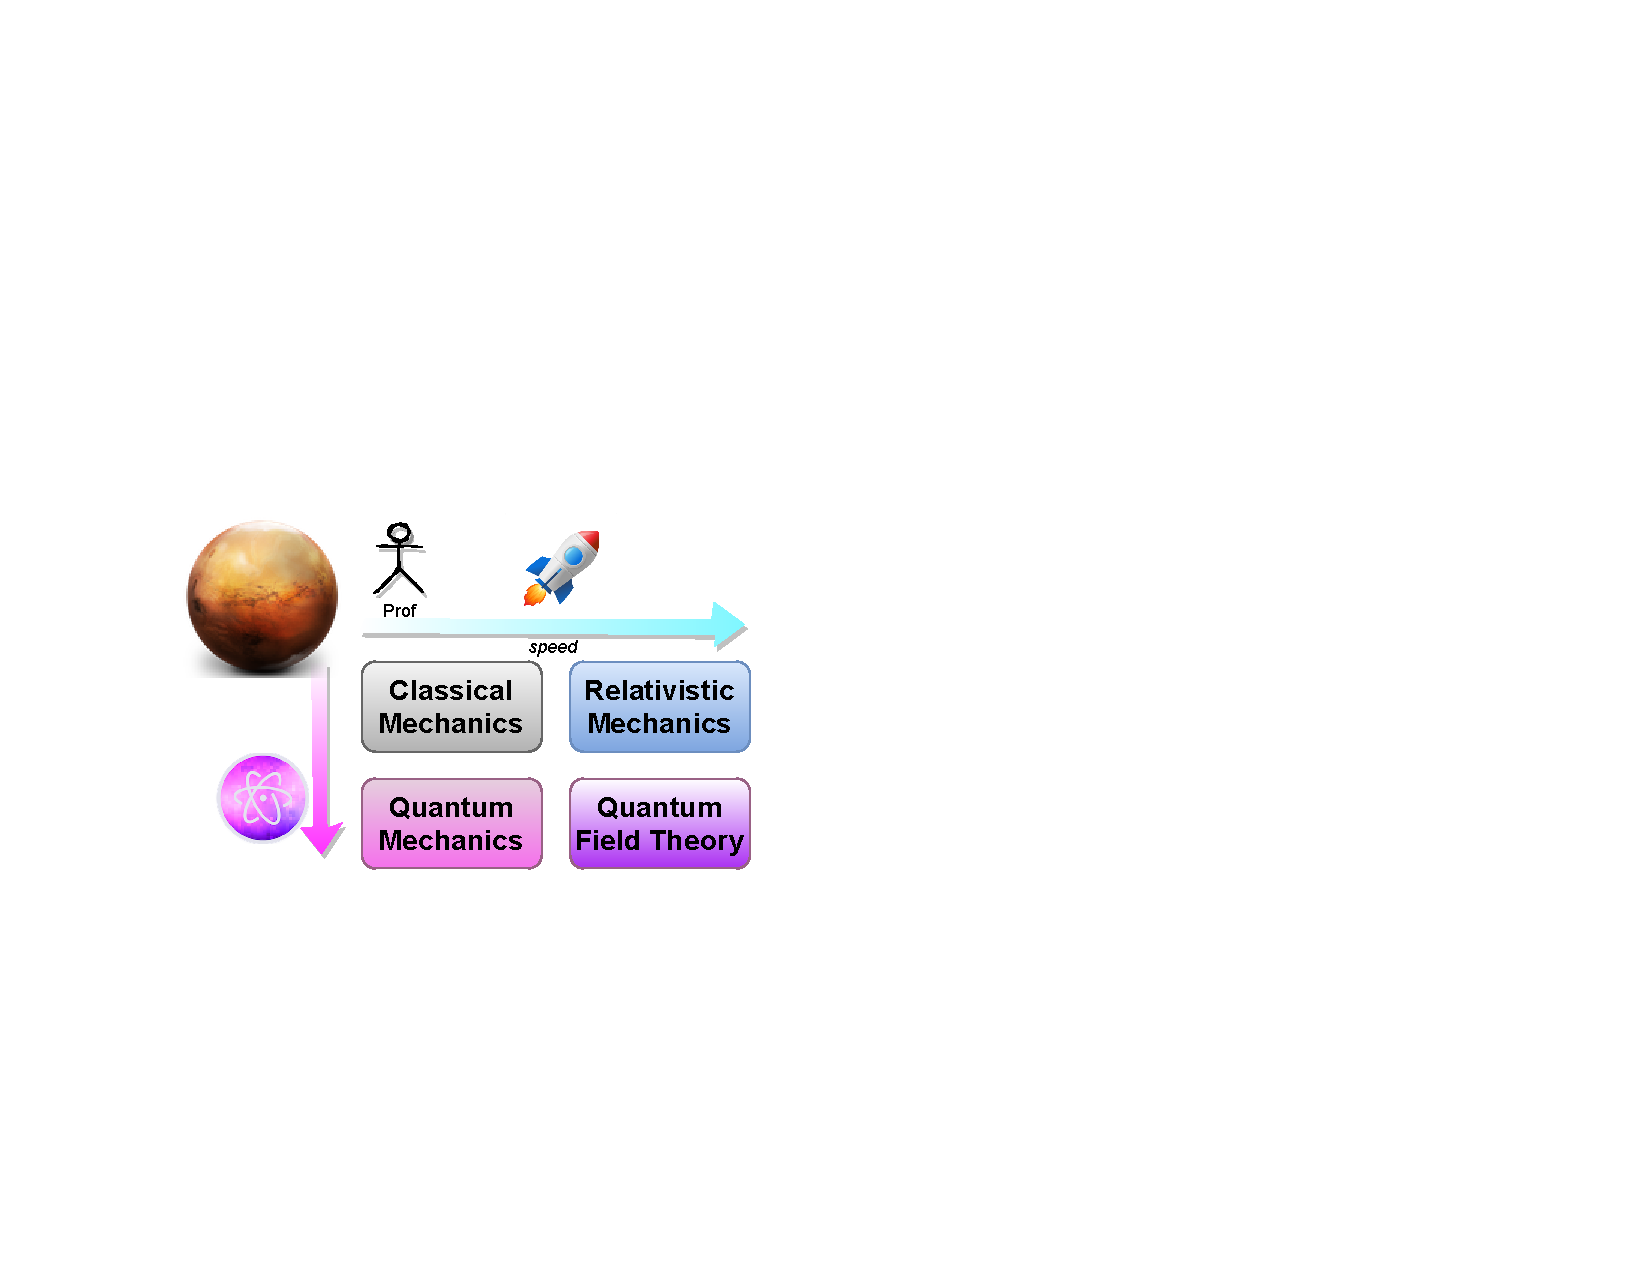
\includegraphics[width=0.7\columnwidth]{stat-mech-overview.pdf}
\caption{Statistical Mechanics covers all physical phenomena. In this class we will mainly cover the low speed cases, with a few mildly relativistic examples (e.g. Blackbody radiation and the Ultraviolet Catastrophe).}
\end{figure}
